%---------
% place your email id between the braces so that your homework has a name
\def\yourname{Mark Xiong}
% -----------------------------------------------------
\def\duedate{4/12/24}
\def\duelocation{via \href{https://www.gradescope.com/courses/753885}{Gradescope}}
\def\hnumber{4}
\def\prof{Lorenzo Orecchia}
\def\course{\href{https://canvas.uchicago.edu/courses/56880}{CMSC 27200 - Spring 2024}}
%-------------------------------------

\documentclass[10pt]{article}
\usepackage[colorlinks,urlcolor=blue]{hyperref}
\usepackage[osf]{mathpazo}
\usepackage{amsmath,amsfonts,graphicx}
\usepackage{latexsym}
%\usepackage{subfig}
\usepackage{algpseudocode}
\usepackage[shortlabels]{enumitem}
\usepackage{algorithm}
\usepackage{listings}

\usepackage{tikz}
\usepackage{qtree}
\usepackage{tikz-qtree}
\usepackage{subcaption}
\usepackage{float}   

%\usepackage[top=1in,bottom=1.4in,left=1.5in,right=1.5in,centering]{geometry}
\usepackage{fullpage}
\usepackage{color}
\definecolor{mdb}{rgb}{0.3,0.02,0.02} 
\definecolor{cit}{rgb}{0.05,0.2,0.45}
\usepackage{wrapfig}
%\pagestyle{myheadings}
\markboth{\yourname}{\yourname}

\thispagestyle{empty}

\newenvironment{proof}{\par\noindent{\it Proof.}\hspace*{1em}}{$\Box$\bigskip}
\newcommand{\qed}{$\Box$}
\newcommand{\alg}[1]{\mathsf{#1}}
\newcommand{\handout}{
   \renewcommand{\thepage}{H\hnumber-\arabic{page}}
   \noindent
   \begin{center}
      \vbox{
    \hbox to \columnwidth {\sc{\course} --- \prof \hfill}
    \vspace{-2mm}
    \hbox to \columnwidth {\sc due \MakeLowercase{\duedate} \duelocation\hfill {\Huge\color{mdb}H\hnumber.\yourname}}
      }
   \end{center}
   \vspace*{2mm}
}
\newcommand{\solution}[1]{
\vspace{2mm}

\noindent Collaborators:

\vspace{5mm}

\medskip\noindent{\color{cit}\textbf{Solution:} #1}}

\newcommand{\bit}[1]{\{0,1\}^{ #1 }}
\newcommand{\extraspace}{\medskip\noindent{\color{cit} Extra space for your solution}\newpage}
%\dontprintsemicolon
%\linesnumbered=
\newtheorem{problem}{\sc\color{cit}Problem}
\newtheorem{lemma}{Lemma}
\newtheorem{theorem}{Theorem}
\newtheorem{definition}{Definition}
\newtheorem{claim}{Claim}


\begin{document}
\handout
\begin{itemize}
\item The assignment is due at Gradescope on \duedate.

\item A LaTeX template will be provided for each homework. You are strongly encouraged to type your homework into this template using \LaTeX.  If you are writing by hand, please fill in the solutions in this template, inserting additional sheets as necessary. This will help facilitate the grading.

\item You are permitted to discuss the problems with up to 2 other students in the class (per problem); however, {\em you must write up your own solutions, in your own words}. Do not submit anything you cannot explain. If you do collaborate with any of the other students on any problem, please list all your collaborators in the appropriate spaces.

\item Similarly, please list any other source you have used for each problem, including other textbooks or websites.

\item {\em Show your work.} Answers without justification will be given little credit.

\item Your homework is \textit{resubmittable}. Please refer to the course syllabus on Canvas for a more detailed description of this. For any problem that you have not changed from your last submission, please make sure to indicate this in your submission to help our graders grade faster. 

\item Is anyone still reading these?

\end{itemize}

%%%%%%%%%%%%%%%%%%%%%%%%%%%%%%%%%%%%%%%%%%%

%%%%%%%%%%%%%%%%%%%%%%%%%%%%%%%%%%%%%%%%%%%

\newpage
\begin{problem}[Linear Algebra Practice]
This question is on the basics of linear algebra, please write out all steps for computation and formal proofs:
\begin{enumerate}[(a)]
    \item Let $A = \begin{pmatrix} 2 & 5 \\ 1 & 3 \end{pmatrix}$, compute the following:
    \begin{enumerate}[(i)]
        \item $A^{-1}$
        \item $A^T$
        \item $A^2$
    \end{enumerate}
    \item Let $A$ and $B$ be $n\times n$ matrices. What's wrong with the equation $(A+B)^2 = A^2 + 2AB + B^2$? Prove that the above equation holds if and only if $A$ and $B$ commute.
    \item Let $A$ be a $n \times m$ matrix. Consider function $f: \mathbb{R}^n \rightarrow \mathbb{R}^m$ where $f(x) = Ax$. Formally prove that $f$ is a linear map (i.e. you need to show that $f(ax+by) = af(x) + bf(y)$ for all $x, y \in \mathbb{R}^n$ and $a, b \in \mathbb{R}$).
\end{enumerate}
    
\end{problem}

\begin{solution} 
The solution to this problem is below.
\begin{enumerate}[(a)]
    \item 
    \begin{enumerate}[(i)]
        \item $A^{-1}$ = $\frac{1}{a\cdot d-b\cdot c}\begin{pmatrix}d & -b \\ -c & a\end{pmatrix} = \frac{1}{2x3-5x1}\begin{pmatrix}3 & -5 \\ -1 & 2\end{pmatrix} = \begin{pmatrix}3 & -5 \\ -1 & 2\end{pmatrix}$
        \item $A^T$ = $\begin{pmatrix}2 & 1 \\ 5 & 3\end{pmatrix}$
        \item $A^2$ = $\begin{pmatrix}2 & 5 \\ 1 & 3\end{pmatrix} \cdot \begin{pmatrix}2 & 5 \\ 1 & 3\end{pmatrix} = \begin{pmatrix}2x2+5x1 & 2x5+5x3 \\ 1x2+3x1 & 1x5+3x3\end{pmatrix} = \begin{pmatrix}9 & 25 \\ 5 & 14\end{pmatrix}$
    \end{enumerate}
    \item Assume $A$ and $B$ commute, then $AB = BA$. Then $(A+B)^2 = (A+B)(A+B) = A^2 + AB + BA + B^2 = A^2 + 2AB + B^2$. Conversely, if $(A+B)^2 = A^2 + 2AB + B^2$, then $AB = BA$, which implies that $A$ and $B$ commute. 
    \item To prove $f$ is a linear map, we need to show the addicitivity and homogeneity properties. Consider $f(x+y) = A(x+y)$, we get $f(x+y) = Ax + Ay = f(x) + f(y)$. Consider $f(ax) = A(ax)$, we can pull the scaler $a$ out and get $f(ax) = a(Ax) = af(x)$. Therefore, $f$ is a linear map.
\end{enumerate}
\end{solution}

\newpage

%%%%%%%%%%%%%%%%%%%%%%%%%%%%%%%%%%%%%%%%%%%

%%%%%%%%%%%%%%%%%%%%%%%%%%%%%%%%%%%%%%%%%%%

\begin{problem}[Modular FFT]
This question is based on problem 2.30 from [DPV].

This problem illustrates how to do the Fourier Transform (FT) in modular arithmetic, for example, modulo 7.
\begin{enumerate}
    \item[(a)] There is at least one number $\omega$ such that all the powers $\omega$, $\omega^2$,..., $\omega^6$ are distinct (modulo $7$). Find one such $\omega$, and show that $\omega$ + $\omega^2$ + · · · + $\omega^6 \equiv 0 \mod 7$. (Interestingly, for any prime modulus there is such a number.)
    \item[(b)] Using the matrix form of the FT, produce the transform of the sequence $(0,1,1,1,5,2)$ modulo $7$; that is, multiply this vector by the $6\times 6$ matrix $M_6(\omega)$, for the value of $\omega$ you found earlier. In the matrix multiplication, all calculations should be performed modulo 7.
    \item[(c)] Write down the matrix necessary to perform the inverse FT. Recall that dividing by a number amounts to multiplying by its inverse. Show that multiplying by this matrix returns the original sequence. (Again all arithmetic should be performed modulo 7.)
    \item[(d)] Now show how to multiply the polynomials $x^2 + x + 1$ and $x^3 + 2x - 1$ using the FT modulo 7.
\end{enumerate}
\end{problem}
\begin{solution}
    The solution to this problem is below.
    \begin{enumerate}[(a)]
        \item $\omega = 3$ is one such number. $\omega + \omega^2 + \omega^3 + \omega^4 + \omega^5 + \omega^6 = 3 + 2 + 6 + 4 + 5 + 1 = 21 \equiv 0 \mod 7$.
        \item Continue the calculations from part (a).\\
        We get the matrix $M_6(\omega)$ is $\begin{pmatrix}1 & 1 & 1 & 1 & 1 & 1 \\ 1 & 3 & 2 & 6 & 4 & 5 \\ 1 & 2 & 4 & 1 & 2 & 4 \\ 1 & 6 & 1 & 6 & 1 & 6 \\ 1 & 4 & 2 & 1 & 4 & 2 \\ 1 & 5 & 4 & 6 & 2 & 3\end{pmatrix} \cdot \begin{pmatrix}0 \\ 1 \\ 1 \\ 1 \\ 5 \\ 2\end{pmatrix} = \begin{pmatrix}10 \\ 41 \\ 25 \\ 30 \\ 31 \\ 31\end{pmatrix} \equiv \begin{pmatrix}3 \\ 6 \\ 4 \\ 2 \\ 3 \\ 3\end{pmatrix} \mod 7$
        \item $M_6(\omega^{-1}) = \begin{pmatrix}
            1 & 1 & 1 & 1 & 1 & 1 \\
            1 & 5 & 4 & 6 & 3 & 2 \\
            1 & 4 & 2 & 1 & 4 & 2 \\
            1 & 6 & 1 & 6 & 1 & 6 \\
            1 & 2 & 4 & 1 & 2 & 4 \\
            1 & 3 & 2 & 6 & 4 & 5
        \end{pmatrix}$  $Inverse$ $FT = 6\cdot M_6(\omega^{-1}) \cdot \begin{pmatrix}3 \\ 6 \\ 4 \\ 2 \\ 3 \\ 3\end{pmatrix} = 6\cdot M_6(\omega^{-1}) \cdot \begin{pmatrix}3 \\ 6 \\ 4 \\ 2 \\ 3 \\ 3\end{pmatrix} = \begin{pmatrix} 21 \\ 76 \\ 55 \\ 76 \\ 51 \\ 68\end{pmatrix} \equiv \begin{pmatrix}
            0 \\ 1 \\ 1 \\ 1 \\ 5 \\ 2 \end{pmatrix} \mod 7$ 
        \item To multiply the polynomials $x^2 + x + 1$ and $x^3 + 2x - 1$, we first represent them as vectors $(1, 1, 1, 0, 0, 0)$ and $(6, 2, 0, 1, 0, 0)$. FFT of the vector $(1, 1, 1, 0, 0, 0)$ is 
        $\begin{pmatrix}1 & 1 & 1 & 1 & 1 & 1 \\ 1 & 3 & 2 & 6 & 4 & 5 \\ 1 & 2 & 4 & 1 & 2 & 4 \\ 1 & 6 & 1 & 6 & 1 & 6 \\ 1 & 4 & 2 & 1 & 4 & 2 \\ 1 & 5 & 4 & 6 & 2 & 3\end{pmatrix} \cdot$ $\begin{pmatrix}1 \\ 1 \\ 1 \\ 0 \\ 0 \\ 0\end{pmatrix} \equiv \begin{pmatrix}3 \\ 6 \\ 0 \\ 1 \\ 0 \\ 3\end{pmatrix}  \mod 7$. 
        Similarly, FFT of the vector $(6, 2, 0, 1, 0, 0)$ is $\begin{pmatrix}2 \\ 4 \\ 4 \\ 3 \\ 1 \\ 1\end{pmatrix}$. The product of the two polynomials is the product of the two FFTs, 
        which is $\begin{pmatrix}3 \\ 6 \\ 0 \\ 1 \\ 0 \\ 3\end{pmatrix} \cdot \begin{pmatrix}2 \\ 4 \\ 4 \\ 3 \\ 1 \\ 1\end{pmatrix} \equiv \begin{pmatrix}6 \\3 \\ 0 \\ 3 \\ 0 \\ 3\end{pmatrix}$. 
        We need to calculate the final result by inversing the FFT, this gives us 
        $6 \cdot \begin{pmatrix}
            1 & 1 & 1 & 1 & 1 & 1 \\
            1 & 5 & 4 & 6 & 3 & 2 \\
            1 & 4 & 2 & 1 & 4 & 2 \\
            1 & 6 & 1 & 6 & 1 & 6 \\
            1 & 2 & 4 & 1 & 2 & 4 \\
            1 & 3 & 2 & 6 & 4 & 5
        \end{pmatrix} \cdot \begin{pmatrix}6 \\3 \\ 0 \\ 3 \\ 0 \\ 3\end{pmatrix} \equiv \begin{pmatrix}-1 \\1 \\ 1 \\ 3 \\ 1 \\ 1\end{pmatrix} \mod 7$. Therefore, the final result is $x^5 + x^4 + 3x^3 + x^2 + x + 6$.
    \end{enumerate}

\end{solution}

\newpage


%%%%%%%%%%%%%%%%%%%%%%%%%%%%%%%%%%%%%%%%%%%

%%%%%%%%%%%%%%%%%%%%%%%%%%%%%%%%%%%%%%%%%%%

\begin{problem}[Bipartite Graphs]
This question is similar to question 3.7 in [DPV].

A bipartite graph is an undirected graph $G=(V,E)$ whose vertex set $V$ can be partitioned into two sets $V_1$ and $V_2$ (i.e. $V = V_1 \cup V_2$ and $V_1 \cap V_2 = \emptyset$) such that there are no edges between vertices of the same set. In other words, all edges are of the form $(u,v)$, where $u \in V_1$ and $v \in V_2$.

\begin{enumerate}
    \item[(a)]Sketch a proof that a graph is bipartite if and only if it contains no odd cycle.
    \item[(b)]Give an $O(|V|+|E|)$ time algorithm with pseudocode to check if a graph is bipartite, and formally prove that it is correct and that it runs in $O(|V|+|E|)$ time. 
\end{enumerate}
\end{problem}
\begin{solution}
    The solution goes below:
    \begin{enumerate}[(a)]
        \item  To prove the if part, we can divide the graph into two sets $V_1$ and $V_2$ such that there are no edges between vertices of the same set. 
        Consider any cycle in $G$. Start traversing the cycle from any vertex $v$ in $V_1$. The next vertex in the cycle must be in $V_2$, and the one after that back in $V_1$, and so on. When you return to the starting vertex to complete the cycle, you must have made an even number of transitions,
         since we started in $V_1$ and need to end in $V_1$. Therefore, any cycle in $G$ must be even, and therefore $G$ contains no odd cycle. To prove the only if part, we can show that if a graph contains an odd cycle, then it is not bipartite.
         Assume graph $G$ contains no odd cycles. We need to demonstrate that $G$ can be bipartitioned into two sets such that no two adjacent vertices belong to the same set. Choose an arbitrary vertex $v$ and assign it to $V_1$. For everyother vertex $u$ that is reachable from $v$ by an odd-length path, assign it to $V_2$. For every vertex $u$ that is reachable from $v$ by an even-length path, assign it to $V_1$. 
         This is a valid bipartition. Consider edge $uw$. Suppose both $u$ and $w$ are in $V_1$. Then the path from $w$ to $u$ is odd. But since $uw$ is an edge, and their direct connections implies an even-length path, which is a contradiction. The same applies to $V_2$. Therefore, $G$ is bipartite as if any edge exists between $u$ and $w$, they must be in separete sets.
        \begin{algorithm}
            \caption{Check if a graph is bipartite} 
            \begin{algorithmic}[1]
            \Statex \textbf{Input:} Graph $G=(V,E)$
            \Statex \textbf{Output:} True if the graph is bipartite, False otherwise
            \State Adjecency lists $adj$ = V*[[ ]]
            \State for all (u, v) in $E$: adj[u].append(v), adj[v].append(u)
            \State colors = [V*-1]
            \State queue = []
            \State for i in V: 
                \If{i is not colored} 
                    \State  color i with 0
                    \State add i to queue
                    \While {queue is not empty}
                        \State currentVertex = queue.pop(0)
                        \For {v in adj[currentVertex]}
                            \If {v is not colored}
                                \State color v with the opposite color of currentVertex
                                \State add v to queue
                            \ElsIf {v has the same color as currentVertex}
                                \State \Return False
                            \EndIf
                        \EndFor
                    \EndWhile
                \EndIf \\
            \Return True
            \end{algorithmic}
        \end{algorithm}
    \end{enumerate}
    The proof of correctness goes as following: The algorithm checks if a graph is bipartite by coloring the vertices with two colors. For each uncolored vertex, the algorithm assigns a color and adds it to the queue, then proceeds with a BFS to color each adjacent vertex
    with the opposite color. If the algorithm encounters an adjacent vertex that is already colored with the same color as the current vertex, then the graph is not bipartite because it added another step to the even number of steps we've gone through, so it gives odd steps. Any closed walk that traces through an odd number of edges would require switching colors an odd number of times, which is impossible if it starts and ends with the same vertex with the same color,
    and therefore returns false because it implies that we find an odd-length cycle in the graph, which contradicts the definition of bipartite graph. For the adjecent verteces with the opposite color, it skips over and proceeds to the next vertex in queue.
    If the algorithm successfully colors all vertices with the two colors without a conflict, it returns True.
    \\ \\
    The time complexity of the algorithm is $O(|V|+|E|)$. The algorithm initializes the adjacency list in $O(|E|)$ time, colors the vertices in $O(|V|)$ time, as each vertex is added to queue once and colored once. Therefore, the total time complexity is $O(|V|+|E|)$.
\end{solution}
\newpage

%%%%%%%%%%%%%%%%%%%%%%%%%%%%%%%%%%%%%%%%%%%

%%%%%%%%%%%%%%%%%%%%%%%%%%%%%%%%%%%%%%%%%%%

\begin{problem}[Verifying Binary Search Trees]
For this problem you may assume that a binary tree node is defined as follows:

\begin{verbatim}
class node:
    left: node = None
    right: node = None
    value
\end{verbatim}
You can assume that the values are distinct and the value type supports comparison.
A binary tree $T$ is called a binary search tree (BST) if and only if \textbf{for every node V} in the tree
\[\max_{U \in V.left} U.val < V.val < \min_{W \in V.right} W.val\]

\begin{enumerate}[(a)]
    \item Write pseudocode for a \textbf{recursive} algorithm that takes as input the root $T$ of a binary tree and returns whether it is a BST. Your algorithm can optionally return more than just a boolean value. You are allowed to define helper functions if you want. Your algorithm should run in $O(n)$ time, where $n$ is the number of nodes in tree $T$.

    \item Prove the correctness of your algorithm.
\end{enumerate}
The height of a tree is defined as 
\[height(T) = \begin{cases} 0 & T = None \\
1 + \max\big(height(T.left), height(T.right)\big) & \text{o.w.}\end{cases}\]
We would like all our Binary Search Trees operations (look-up, insertion, deletion) to have $O(\log n)$ time complexity. To achieve that, we require the BST to also be \textbf{balanced}.
A BST is balanced if and only if \textbf{for every node V} in the tree
\[\big|height(V.left) - height(V.right)\big| \leq 1\]

\begin{enumerate}[(a),resume]
    \item Modify below your pseudocode from part (a) to check if the binary tree $T$ is a \textbf{balanced} BST. Your modified algorithm should also have $O(n)$ time complexity.
\end{enumerate}
\end{problem}

\begin{figure}[ht]
    \centering
    \begin{subfigure}[b]{0.3\textwidth}
        \centering
        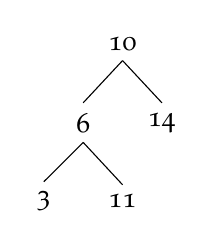
\begin{tikzpicture}[level distance=1cm,
                            level 1/.style={sibling distance=1cm},
                            level 2/.style={sibling distance=1cm}]
            \node {10}
                child {node {6}
                    child {node {3}}
                    child {node {11}}
                }
                child {node {14}};
        \end{tikzpicture}
        \caption{This is not a BST since $11 > 10$}
    \end{subfigure}
    \begin{subfigure}[b]{0.3\textwidth}
        \centering
        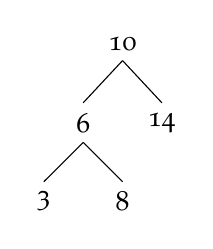
\begin{tikzpicture}[level distance=1cm,
                            level 1/.style={sibling distance=1cm},
                            level 2/.style={sibling distance=1cm}]
            \node {10}
                child {node {6}
                    child {node {3}}
                    child {node {8}}
                }
                child {node {14}};
        \end{tikzpicture}
        \caption{This is a balanced BST}
    \end{subfigure}
    \begin{subfigure}[b]{0.3\textwidth}
        \centering
        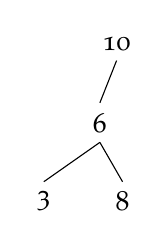
\begin{tikzpicture}[level distance=1cm,
                            level 1/.style={sibling distance=1cm},
                            level 2/.style={sibling distance=1cm}]
            \node {10}
                child[left] {node {6}
                    child {node {3}}
                    child {node {8}}
                };
        \end{tikzpicture}
        \caption{This is a BST, but not balanced}
    \end{subfigure}
\end{figure}

\begin{solution}
    The solution goes below:
    \begin{enumerate}[(a)]
        \item The algorithm is as follows:
        \begin{algorithm}
            \caption{Check if a binary tree is a BST} 
            \begin{algorithmic}[1]
            \Statex \textbf{Input:} Root node $T$ of a binary tree
            \Statex \textbf{Output:} True if the tree is a BST, False otherwise
            \Function{isBST}{node T, Min, Max} (helper function)
                \If{T is None}
                    \State \Return True
                \EndIf
                \If{(Min is not None and T.value $\leq$ Min) or (Max is not None and T.value $\geq$ Max)}
                    \State \Return False
                \EndIf
                \State \Return isBST(T.left, Min, T.value) and isBST(T.right, T.value, Max)
            \EndFunction
            \Function{verifyBST}{node T}
                \State \Return isBST(T, None, None)
            \EndFunction
            \end{algorithmic}
        \end{algorithm}
        \\ \\
        \item \textbf{Base Case:} If the root node is None, the algorithm returns True because there're no nodes to violate the BST properties. \\
        \textbf{Inductive Step:} Assume that for all k < n, where k is the number of nodes in any subtree, the function correctly determines whether the subtree is a BST.
        The algorithm checks if the current node violates the BST properties by comparing the value of the current node with the Min and Max values. If the current node violates the BST properties, the algorithm returns False. Otherwise, the algorithm recursively checks the left and right subtrees with the updated Min and Max values. If both subtrees are BSTs, the algorithm returns True. Therefore, the algorithm is correct.
        As each node is visited once, the time complexity of the algorithm is $O(n)$.
        \item The modified algorithm is as follows:
         \begin{algorithm}
            \caption{Check if a binary tree is a BST} 
            \begin{algorithmic}[1]
            \Statex \textbf{Input:} Root node $T$ of a binary tree
            \Statex \textbf{Output:} True if the tree is a Balanced BST, False otherwise
            \Function{isBalancedBST}{node T} (helper function)
                \If{T is None}
                    \State \Return True, 0
                \EndIf
                \State  leftIsBalanced, leftHeight = isBalancedBST(T.left)
                \If{not leftIsBalanced}
                    \State \Return False, 0
                \EndIf
                \State rightIsBalanced, rightHeight = isBalancedBST(T.right)
                \If{not rightIsBalanced}
                    \State \Return False, 0
                \EndIf
                \State \Return True, 1 + max(leftHeight, rightHeight)
            \EndFunction
            \Function{verifyBalancedBST}{node T}
                \State isBalanced, height = isBalancedBST(T)
                \State \Return isBalanced
            \EndFunction
            \end{algorithmic}
        \end{algorithm}
    \end{enumerate}
\end{solution}

\end{document}